%%
%% This is file `./samples/longsample.tex',
%% generated with the docstrip utility.
%%
%% The original source files were:
%%
%% apa7.dtx  (with options: `longsample')
%% ----------------------------------------------------------------------
%% 
%% apa7 - A LaTeX class for formatting documents in compliance with the
%% American Psychological Association's Publication Manual, 7th edition
%% 
%% Copyright (C) 2021 by Daniel A. Weiss <daniel.weiss.led at gmail.com>
%% 
%% This work may be distributed and/or modified under the
%% conditions of the LaTeX Project Public License (LPPL), either
%% version 1.3c of this license or (at your option) any later
%% version.  The latest version of this license is in the file:
%% 
%% http://www.latex-project.org/lppl.txt
%% 
%% Users may freely modify these files without permission, as long as the
%% copyright line and this statement are maintained intact.
%% 
%% This work is not endorsed by, affiliated with, or probably even known
%% by, the American Psychological Association.
%% 
%% ----------------------------------------------------------------------
%% 
\documentclass[man]{apa7}

\usepackage{lipsum}

\usepackage[american]{babel}

\usepackage{caption} % For captioning outside figures
\usepackage{capt-of} % For captioning outside figures

\usepackage{siunitx}

\usepackage{csquotes}
\usepackage[style=apa,backend=biber]{biblatex}
\addbibresource{bibliography.bib}

\title{Parking Occupancy Detection from CCTV Images}
\shorttitle{}
\authorsnames{Jule Valendo Halim -1425567}
\authorsaffiliations{GEOM90038 - Advanced Imaging}

\begin{document}

\maketitle
\tableofcontents
\newpage
\section{Introduction}

Recent developments in data has undergone significant changes from data processing into machine learning due to increased volumes of readily available data (\textcite{KHAN20201444}). The introduction of image-based neural network architecture has allowed the field of computer vision to flourish. Computer vision leverages the power of machine learning to derive meaningful information from visual data, which allows them to take actions and recommendations when they detect issues. Powerful advances in machine learning such as the widely popular transformer model that Chat-GPT is based on has also been adapted to be trained on visual information (\textcite{elnouby2021training}). Figure \ref{fig:representationNeuralNetwork} provides a representation of a neural network, which consists of multiple layers. The input layer is the initial data, and hidden layers calculate the weights of each of these data and propagates them forward to other hidden layers. Finally, the output layer provides probabilities of the desired output (e.g., some classification label).

\begin{minipage}{\linewidth}
  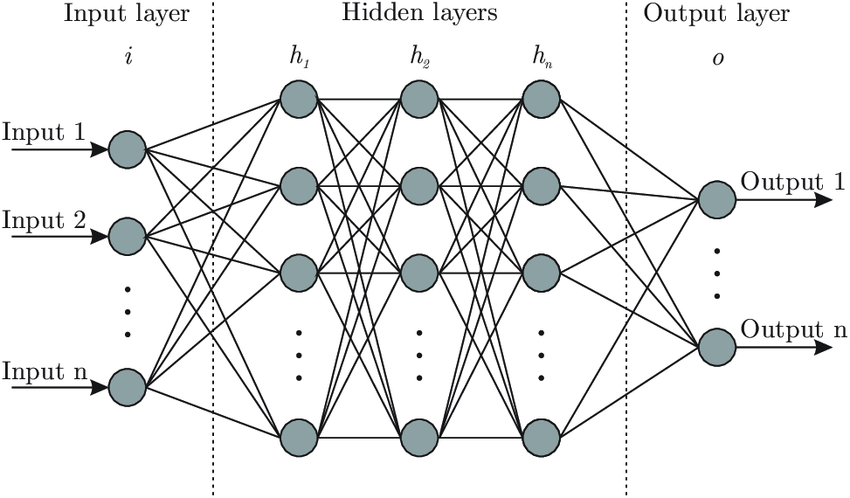
\includegraphics[height=\textheight/4 ,width=\textwidth/1]{figures/sampleNeuralNetwork.png}
  \captionof{figure}{Visual Representation of Layers That Makes Up a Neural Network (\textcite{neuralNetwork})}
  \label{fig:representationNeuralNetwork}
\end{minipage}

Figure \ref{fig:exampleArchitecture} provides a simplified neural network architecture for visual data. The visual data that is placed into the input layer depends on the specific architecture and design. In the case of figure \ref{fig:exampleArchitecture}, a section of the image is placed into the input layer. It is then propagated forward towards additional layers before finally obtaining the results of the output layer, which in this case, attempts to classify the image into four possible species.

\begin{minipage}{\linewidth}
  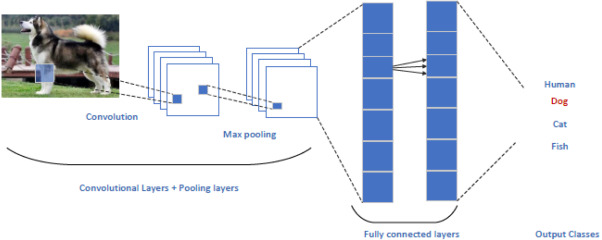
\includegraphics[height=\textheight/4 ,width=\textwidth/1]{figures/exampleML.jpg}
  \captionof{figure}{Sample Architecture of Machine Learning Being Used in Computer Vision (\textcite{CHAI2021100134})}
  \label{fig:exampleArchitecture}
\end{minipage}

The use of computer vision has been applied to wide range of different fields. For example, \textcite{MEDICAL} discussed the way medical imaging applications in multiple medical areas such as pathology and dermatology has enhanced the level of care provided. Another field in which machine learning has enhanced computer vision is in the automation and digitization of fruit quality measuring and maintainence (\textcite{SUPERMARKET}). Figure \ref{fig:exampleDetection} shows how computer vision can be used to detect cars and humans in images. These detections are generated post-training, where multiple images are provided for training the neural network. The trained neural network can then be given new images or even real time video to detect what they were trained to. However, as seen in figure \ref{fig:exampleDetection}, such neural networks are not perfect, and can misclassify or not detect parts of the image that they are supposed to (e.g., the model did not successfully classify one of the humans walking).

\newpage

\begin{minipage}{\linewidth}
  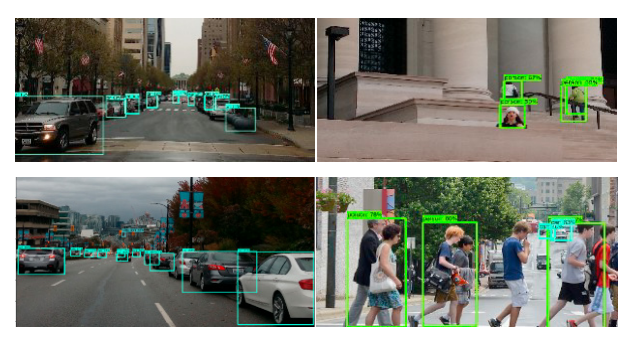
\includegraphics[height=\textheight/4 ,width=\textwidth/2]{figures/detectionExample.png}
  \captionof{figure}{Sample Image Detection Results of Cars and People Using Deep Learning and RCNN Models(\textcite{KHAN20201444})}
  \label{fig:exampleDetection}
\end{minipage}

Faster Recurrent Neural Network models (FasterRCNN model) are a form of neural network that can detect objects in images. The FasterRCNN model is based off \textcite{fasterRCNN}. It consists of two main components, the Region Proposal Network (RPN) and the FastRCNN. RPNs are a convolutional neural network, which are a form of neural network such as those described above, but are specialized in taking three dimensional data (such as images) as inputs. RPNs are further specialized to handle different schemas of different images. Figure \ref{fig:RPN} shows the different schemas that the RPN can handle, namely differing scales, differing filter sizes, and multiple references of the same image. 

\begin{minipage}{\linewidth}
  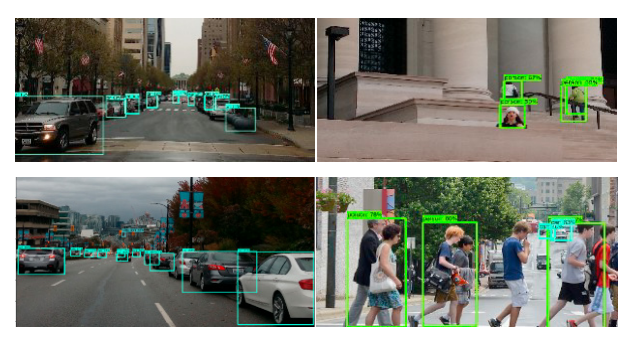
\includegraphics[height=\textheight/4 ,width=\textwidth/2]{figures/detectionExample.png}
  \captionof{figure}{Different Schemas that RPNs Are Adapted To(\textcite{fasterRCNN})}
  \label{fig:RPN}
\end{minipage}

The other component, the FastRCNN (\textcite{fastRCNN}) is a neural network that has been shown to be much faster than other image detection neural networks. The main innovation that causes this increased detection speed is the use of of Regions of Interest (RoI). The RoI is defined with a four-tuple (r,c,h,w). The r and c specifies the top-left corner, while the h and w defines its height and width respectively. These tuples are then max-pooled to convert features inside regions of interest into a small feature map with fixed spatial size (e.g., height and width of 6 x 7). Figure \ref{fig:ROI} shows the overall architecture of the fastRCNN. As seen in this figure, the image is projected into an RoI format before being pooled and trained on a neural network.

\begin{minipage}{\linewidth}
  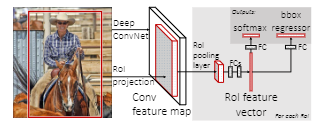
\includegraphics[]{figures/ROI.png}
  \captionof{figure}{The FastRCNN Architecture, Including the Conversion of Images into ROI(\textcite{fastRCNN})}
  \label{fig:ROI}
\end{minipage}

The FasterRCNN architecture has layers that provide output towards the RPN. This is then used to create a proposal, which basically proposes what sort of schema the image is using (see figure \ref{fig:RPN}). The image that is passed through the RPN is also used to create feature maps, which create is then passed to the the RoI pooling before being passed to a classifier. In this architecture, the RPN is performing the 'attention' task of FasterRCNN. Attention allows the model to incorporate sequential information into the model (e.g., in a picture of a man on a horse, the model is able to remember that the section of the image with a hat is in the upper-middle area of the whole image). Figure \ref{fig:fasterRCNNArchitecture} shows the entirety of the FasterRCNN architecture.

\begin{minipage}{\linewidth}
  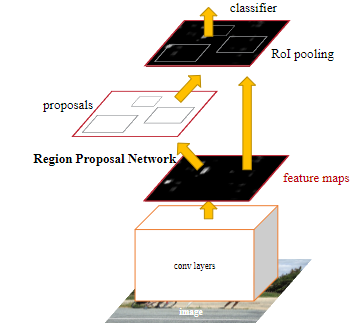
\includegraphics[height=\textheight/4 ,width=\textwidth/2]{figures/fasterRCNN2.png}
  \captionof{figure}{The FasterRCNN Architecture, Showing the Components of RPN and FastRCNN RoI (\textcite{fasterRCNN})}
  \label{fig:fasterRCNNArchitecture}
\end{minipage}

The other model used in this report is the Resnet50 CNN model (\textcite{resnet50}). The Resnet50 CNN model's building block consists of a series of weight layers that have an relu activation function (an activation function converts the weights provided by the layer mapped to an output). Relu takes the maximum of two values and returns an output depending on the input (e.g., a relu that is max(0,x) and has a binary classification task to classify 0 and 1 would classify an output as 1 if x is greater than 0, and classify it as 0 if it is less than 0). Figure \ref{fig:resnet50} shows the building block layer of the Resnet50. The Resnet50 CNN consists of multiple of these layers along with other kinds of layers, one of which is the max-pool layer. This increased depth of representation is vital for visual recognition tasks, and this model is popular in many visual recognition tasks.

\begin{minipage}{\linewidth}
  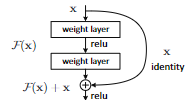
\includegraphics[height=\textheight/6 ,width=\textwidth/4]{figures/resnet.png}
  \captionof{figure}{The Resnet50 CNN Building Block (Layer)(\textcite{resnet50})}
  \label{fig:resnet50}
\end{minipage}

In this report, I aim to use and investigate a pre-trained FasterRCNN model and Resnet50 CNN model(trained on the PKPlot dataset) to detect cars and delineate parking spaces in a picture of the Barry Street parking lot. The software used will be MATLAB 2020a, along with additional toolboxes such as the deep learning toolbox. The methodology of this begins with a visualization of the dataset, before using a pre-trained Resnet50 CNN classifier to identify whether a parking slot is occupied or empty. Afterwards, parking slot delineation is done using FasterRCNN, which detects cars. The dataset for this step involves images of the parking slot and bounding boxes, which identifies the space in which an object is identified (see figure \ref{fig:exampleDetection}, where cars and human areas and identified using bounding boxes).

These results will then be evaluated by calculating recall, precision and accuracy. Afterwards, the object performance will be post-processed to improve the resulting classification. Visual inspection of the resulting bounding boxes will also be compared to the ground truth of where bounding boxes should be. Additional information is found in the methods and results section.

\newpage

\section{Methods and Results}

\subsection{Visualizing Dataset}
This step involves loading in the PKPlot and Barry Street annotated images. These annotations are bounding boxes that are manually set. Figure \ref{fig:datasetImages} shows the annotated images of the PKPlot (left) and Barry Street (right) datasets. The PKPlot dataset consists of over 695,000+ parking space images. For this report, only a segment of the total dataset was used.

\begin{minipage}{\linewidth}
  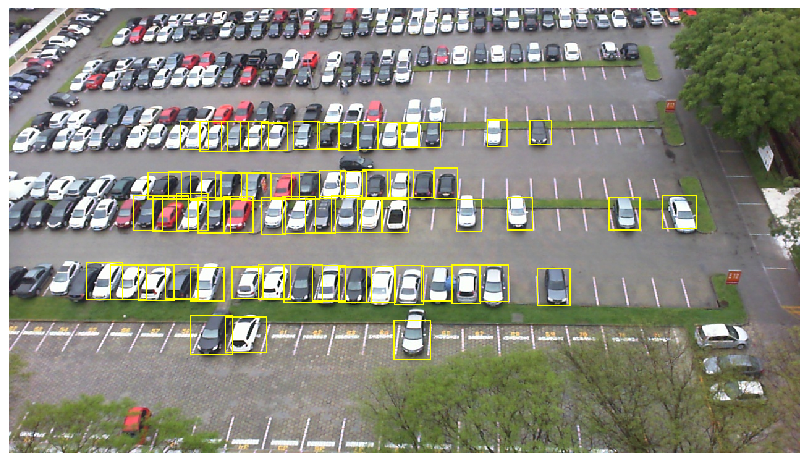
\includegraphics[height=\textheight/4,width=\textwidth/2]{figures/pkplot.png}
  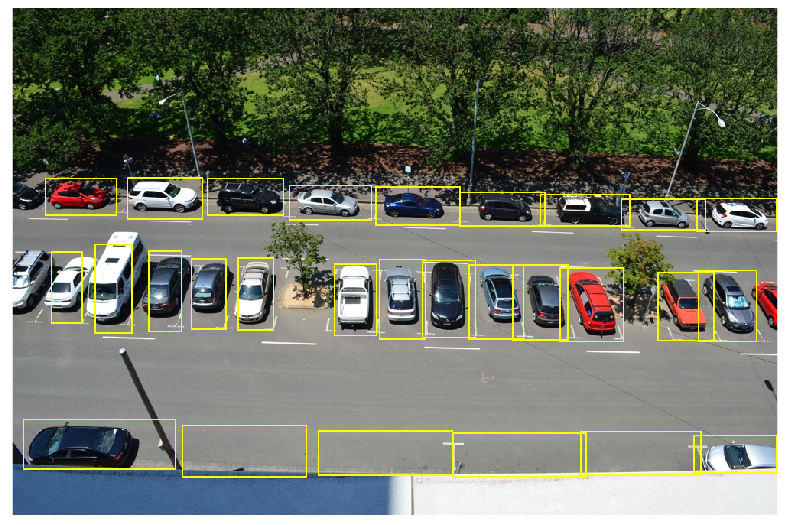
\includegraphics[height=\textheight/4,width=\textwidth/2]{figures/barrystreet.png}
  \captionof{figure}{Images of Annotated from the PKPlot Dataset (left) and Barry Street Dataset (right)}
  \label{fig:datasetImages}
\end{minipage}

Figure \ref{fig:pkplot2} shows a sample empty slot and occupied slot found in the annotated PKPlot datasets.

\begin{minipage}{\linewidth}
  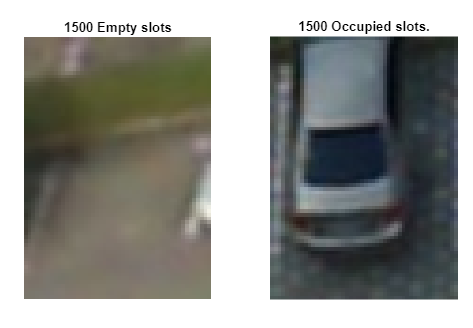
\includegraphics[height=\textheight/4,width=\textwidth/2]{figures/pkplot2.png}
  \captionof{figure}{Sample Image of Empty (left) and Occupied (right) Slots of PKPlot, Sampled From 1500 Empty Spaces and 1500 Occupied Spaces}
  \label{fig:pkplot2}
\end{minipage}


\subsection{Creating Car Detector}

To create the car detector, the pre-trained Resnet50 CNN 

\subsection{Automatic Delineation of Parking Spaces}

\subsection{Evaluation}

\subsection{Post-Processing Improvements}

\section{Discussion}

\subsection{Accuracy, Precision, and Recall Evaluation}

\subsection{Improvement Based on Assumptions}

\subsection{Challenges and Shortcomings}

\subsection{Scopes of Improvement}

\section{Conclusions and Future Directions}

\section{Appendix}

\printbibliography


\end{document}


















% Theoretical overlap is a parameter that is used in fine registration to indicate how many percent of the points are expected to overlap from one another. Multiple values ranging from 10-100\% were tested. However, 30\% was selected as the final value in order to reduce the final RMS.

% The RMS values show great accuracy, with the coarse registration having an RMS of 1.13cm while the fine registration has 2.27cm of final RMS values.


% \begin{minipage}{\linewidth}
%   \small
%   \captionof{table}{Table Showing Statistical Information About C2C Distances with MLS as the Reference Point Cloud}
%   \setlength{\tabcolsep}{3pt} % reduce column spacing
%   \renewcommand{\arraystretch}{0.8} % reduce row spacing
%   \label{tab:RMStable2}
%   \begin{tabular}{@{}llrr@{}}         \toprule
%   \multicolumn{2}{c}{C2C Distance Statistics }        \\ \toprule{}
%   &  MLS as Reference Point Cloud \\ \midrule
%   Mean (m)      & 0.00091 \\
%   Maximum Value (m)       & 1.55\\
%   Minimum Value (m)       & 0  \\ 
%   Max Error (m) & 0.096 \\\bottomrule
%   \end{tabular}
% \end{minipage}

% \vspace{2em}

%  Meanwhile, figure \ref{fig:c2cMLS} shows the visualization of the C2C distances of only overlapping points in both point clouds.

%  \newpage

%  \begin{minipage}{\linewidth}
%   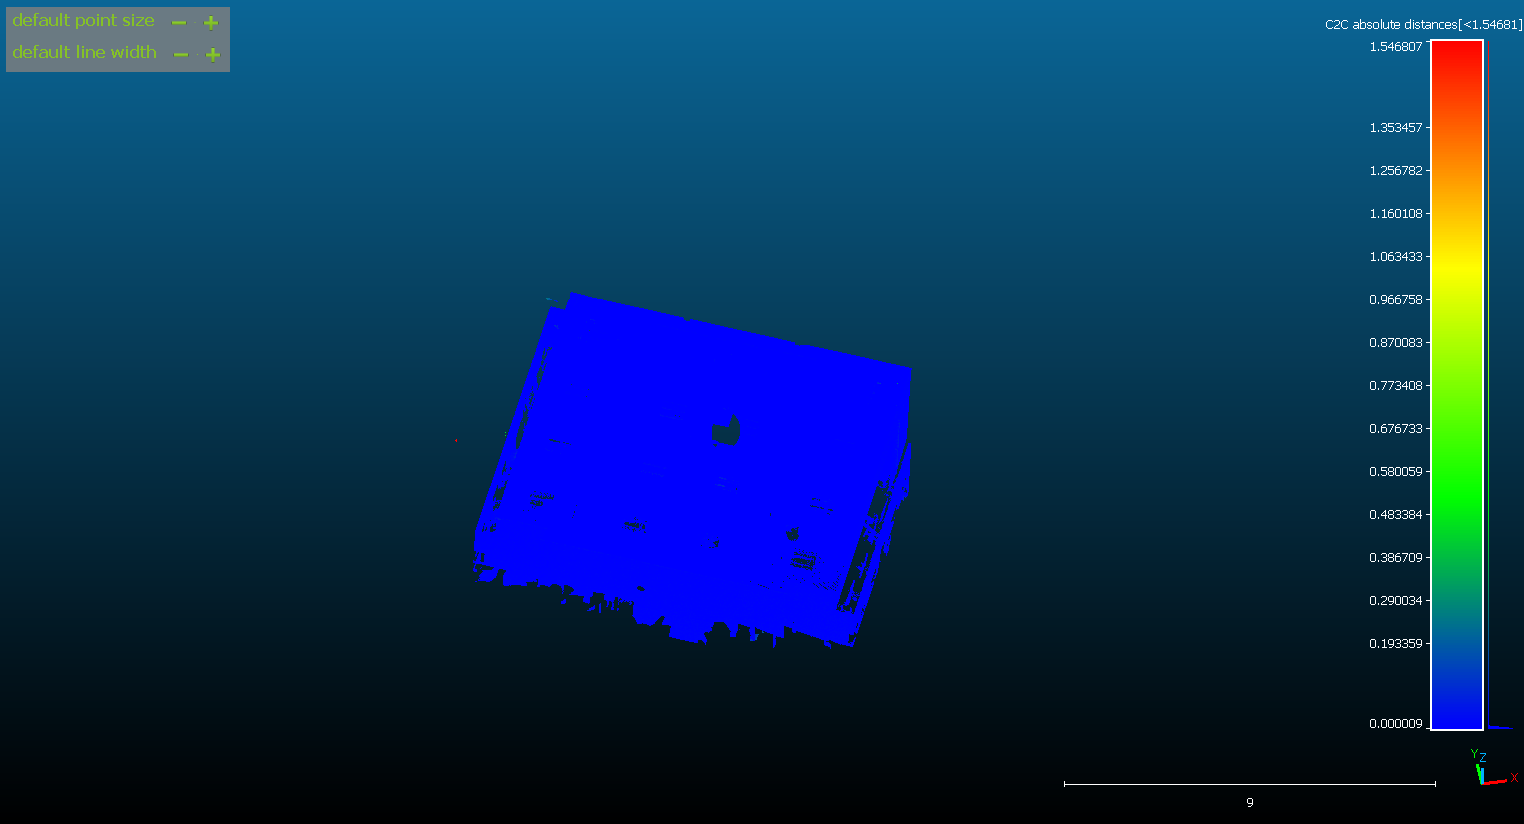
\includegraphics[height=\textheight/2 ,width=\textwidth/1]{figures/MLSasReference.png}
%   \captionof{figure}{C2C Distance Visualization of MLS as the Reference Point Cloud}
%   \label{fig:c2cMLS}
% \end{minipage}

% As seen in figure \ref{fig:c2cMLS} and table \ref{tab:RMStable2}, the areas in which there is only overlap between the TLS and MLS shows very high quality, where there are no outliers involved. This highlights how the TLS is not prone to many outliers. The distances between both point clouds are also on average, about 0.091cm, compared to the C2C distances when outliers were involved, as seen in table \ref{tab:RMStable}, where the means are about 9cm for the area where all distances were considered. This difference could thus be explained by the outliers inflating the means.

% To further investigate these distances, a histogram of the C2C distance was created from the saved text file of the MLS. Figure \ref{fig:c2chistogram} shows the histogram for C2C distances less than or equal to 1 and distances greater than 1. These distances are based on the initial C2C distance calculations in table \ref{tab:RMStable}.

% \begin{minipage}{\linewidth}
%   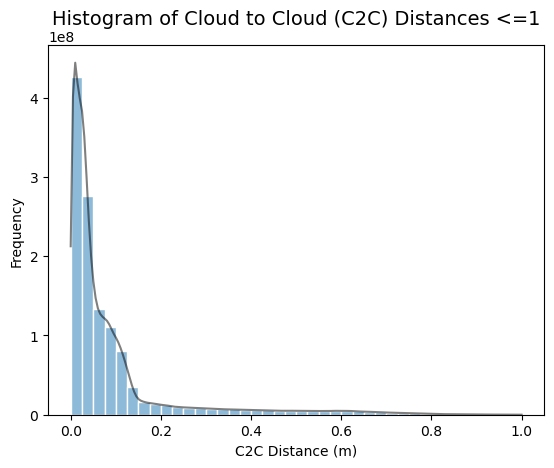
\includegraphics[height=\textheight/4 ,width=\textwidth/2]{figures/MLSC2CHistogramWithLine.png}
%   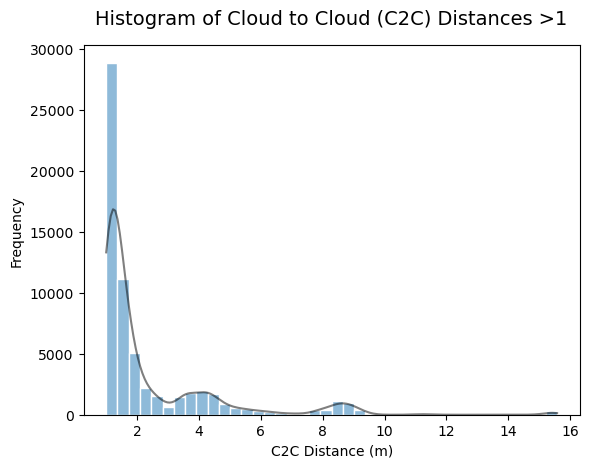
\includegraphics[height=\textheight/4 ,width=\textwidth/2]{figures/MLSC2CHistogramWithLine2.png}
%   \captionof{figure}{Probability distribution of distances less than or equal to 1 (left) and distances higher than 1(right). Note that frequency for the left table is multiplied by \num{1e8}}
%   \label{fig:c2chistogram}
% \end{minipage}



% \begin{minipage}{\linewidth}
%   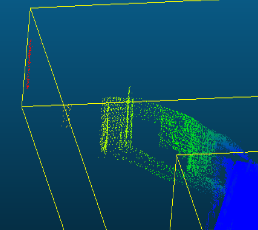
\includegraphics[height=\textheight/4 ,width=\textwidth/2]{figures/grossError.png}
%   \captionof{figure}{Area With Large C2C Distances in the MLS Point Cloud}
%   \label{fig:grossError}
% \end{minipage}


% \end{document}
